\documentclass{beamer}
\usepackage[utf8]{inputenc}
\usetheme{Madrid}
\usecolortheme{default}
\usepackage{amsmath,amssymb,amsfonts,amsthm}
\usepackage{txfonts}
\usepackage{tkz-euclide}
\usepackage{listings}
\usepackage{adjustbox}
\usepackage{array}
\usepackage{tabularx}
\usepackage{gvv}
\usepackage{lmodern}
\usepackage{circuitikz}
\usepackage{tikz}
\usepackage{graphicx}
\setbeamertemplate{page number in head/foot}[totalframenumber]
\usepackage{tcolorbox}
\tcbuselibrary{minted,breakable,xparse,skins}
\definecolor{bg}{gray}{0.95}
\DeclareTCBListing{mintedbox}{O{}m!O{}}{%
  breakable=true,
  listing engine=minted,
  listing only,
  minted language=#2,
  minted style=default,
  minted options={%
    linenos,
    gobble=0,
    breaklines=true,
    breakafter=,,
    fontsize=\small,
    numbersep=8pt,
    #1},
  boxsep=0pt,
  left skip=0pt,
  right skip=0pt,
  left=25pt,
  right=0pt,
  top=3pt,
  bottom=3pt,
  arc=5pt,
  leftrule=0pt,
  rightrule=0pt,
  bottomrule=2pt,
  toprule=2pt,
  colback=bg,
  colframe=orange!70,
  enhanced,
  overlay={%
    \begin{tcbclipinterior}
    \fill[orange!20!white] (frame.south west) rectangle ([xshift=20pt]frame.north west);
    \end{tcbclipinterior}},
  #3,
}
\lstset{
    language=C,
    basicstyle=\ttfamily\small,
    keywordstyle=\color{blue},
    stringstyle=\color{orange},
    commentstyle=\color{green!60!black},
    numbers=left,
    numberstyle=\tiny\color{gray},
    breaklines=true,
    showstringspaces=false,
}
\begin{document}

\title 
{5.5.12}
\date{september 14,2025}


\author 
{Namaswi-EE25BTECH11060}
\frame{\titlepage}
\begin{frame}{Question}
If $\Vec{A}=\begin{pmatrix}
 1 & 1 &  1\\
    1 & 0 &  2\\
    3  & 1 & 1 
\end{pmatrix}$\\find $\Vec{A}^{-1}$ . Hence solve the following system of equations \\
\begin{align*}
   x+y+z=6\\
    x+2z=7\\
    3x+y+z=12 
\end{align*}
\end{frame}
\begin{frame}{Solution}
\begin{align}
\Vec{A} \Vec{x}=\vec{I}
\end{align}
Forming Argumented Matrix
\begin{align}
    \augvec{3}{3}{1 & 1 & 1 & 1 & 0 & 0\\
1 & 0 & 2 & 0 & 1 & 0\\
3 & 1 & 1 & 0 & 0 & 1}
\end{align}
\end{frame}
\begin{frame}{Solution}
    Replace $R2 \to R2-R1$ and $R3 \to R3-3R1 $ \\
\begin{align}
\augvec{3}{3}{1 & 1 & 1 & 1 & 0 & 0\\
0 & -1 & 1 & -1 & 1 & 0\\
0 & -2 & -2 & -3 & 0 & 1} 
\end{align}
Replace $R2 \to -R2$ and $R3 \to R3+2R2 $\\
\begin{align}
    \augvec{3}{3}{ 1 & 0 & 2 & 0 & 1 & 0\\
0 & 1 & -1 & 1 & -1 & 0\\
0 & 0 & -4 & -1 & -2 & 1
}
\end{align}
\end{frame}
\begin{frame}{Solution}
Repalce  \(R_3\leftarrow -\tfrac{1}{4}R_3\)
\begin{align}
    \augvec{3}{3}{1 & 0 & 2 & 0 & 1 & 0\\
0 & 1 & -1 & 1 & -1 & 0\\
0 & 0 & 1 & \tfrac14 & \tfrac12 & -\tfrac14}
\end{align}
Replace \(R_1\leftarrow R_1-2R_3,\; R_2\leftarrow R_2+R_3\)
\begin{align}
    \augvec{3}{3}{1 & 0 & 0 & -\tfrac12 & 0 & \tfrac12\\
0 & 1 & 0 & \tfrac54 & -\tfrac12 & -\tfrac14\\
0 & 0 & 1 & \tfrac14 & \tfrac12 & -\tfrac14}
\end{align} 
\end{frame}
\begin{frame}{Solution}
Thus
\begin{align}
A^{-1}=\begin{pmatrix}
-\tfrac12 & 0 & \tfrac12\\[6pt]
\tfrac54 & -\tfrac12 & -\tfrac14\\[6pt]
\tfrac14 & \tfrac12 & -\tfrac14
\end{pmatrix}.
\end{align}   
\end{frame}
\begin{frame}{Solution}
\begin{align}
   \vec{X}=\vec{A^{-1}} \vec{b}\\
   \vec{X}
   =\begin{pmatrix}
-\tfrac12 & 0 & \tfrac12\\[4pt]
\tfrac54 & -\tfrac12 & -\tfrac14\\[4pt]
\tfrac14 & \tfrac12 & -\tfrac14
\end{pmatrix}
\begin{pmatrix}6\\[2pt]7\\[2pt]12\end{pmatrix}\\
\vec{X}=\begin{pmatrix}
    3 \\ 1 \\ 2
\end{pmatrix}
\end{align}
\end{frame}
\begin{frame}[fragile]
\frametitle{Python Code}
\begin{lstlisting}
    import numpy as np
import matplotlib.pyplot as plt
from mpl_toolkits.mplot3d import Axes3D

# Define the grid
x = np.linspace(-1, 10, 30)
y = np.linspace(-1, 10, 30)
X, Y = np.meshgrid(x, y)
\end{lstlisting}
\end{frame}
\begin{frame}[fragile]
\frametitle{Python Code}
    \begin{lstlisting}
        # Define the planes
Z1 = 6 - X - Y                # From x + y + z = 6
Z2 = (7 - X) / 2              # From x + 2z = 7
Z3 = 12 - 3*X - Y             # From 3x + y + z = 12

# Plot the surfaces
fig = plt.figure(figsize=(10, 7))
ax = fig.add_subplot(111, projection='3d')

    \end{lstlisting}
\end{frame}
\begin{frame}[fragile]
\frametitle{Python Code}
    \begin{lstlisting}
ax.plot_surface(X, Y, Z1, alpha=0.5, color='red', label='x+y+z=6')
ax.plot_surface(X, Y, Z2, alpha=0.5, color='green', label='x+2z=7')
ax.plot_surface(X, Y, Z3, alpha=0.5, color='blue', label='3x+y+z=12')

# Labels
ax.set_xlabel('X')
ax.set_ylabel('Y')
ax.set_zlabel('Z')
ax.set_title('Graph of 3 Planes')

plt.show() 
    \end{lstlisting}
\end{frame}
\begin{frame}[fragile]
\frametitle{C Code}
\begin{lstlisting}
    #include <stdio.h>
#include <math.h>
#define N 3  // Number of variables
int main() {
    int i, j, k;
    float a[N][N+1], ratio;
    float x[N];

    // Augmented matrix input
    // System:
    // x + y + z = 6
    // x + 2z = 7
    // 3x + y + z = 12
    a[0][0] = 1; a[0][1] = 1; a[0][2] = 1; a[0][3] = 6;
    a[1][0] = 1; a[1][1] = 0; a[1][2] = 2; a[1][3] = 7;
    a[2][0] = 3; a[2][1] = 1; a[2][2] = 1; a[2][3] = 12;
\end{lstlisting}   
\end{frame}
\begin{frame}[fragile]
\frametitle{C Code}
\begin{lstlisting}
     // Forward Elimination
    for (i = 0; i < N-1; i++) {
        if (a[i][i] == 0.0) {
            printf("Mathematical Error!\n");
            return 0;
        }
        for (j = i+1; j < N; j++) {
            ratio = a[j][i] / a[i][i];
            for (k = 0; k <= N; k++) {
                a[j][k] -= ratio * a[i][k];
            }
        }
    }

\end{lstlisting}   
\end{frame}
\begin{frame}[fragile]
\frametitle{C Code}
\begin{lstlisting}
    // Back Substitution
    x[N-1] = a[N-1][N] / a[N-1][N-1];
    for (i = N-2; i >= 0; i--) {
        x[i] = a[i][N];
        for (j = i+1; j < N; j++) {
            x[i] -= a[i][j] * x[j];
        }
        x[i] /= a[i][i];
    }
    // Display solution
    printf("Solution:\n");
    for (i = 0; i < N; i++) {
        printf("x[%d] = %.2f\n", i+1, x[i]);
    }
    return 0;
}
\end{lstlisting}   
\end{frame}
\begin{frame}[fragile]
\frametitle{C and Python Code}
\begin{lstlisting}
    import ctypes
import numpy as np

# Load the shared library
lib = ctypes.CDLL('./libgauss.so')

# Define return type and argument types
lib.gauss_elimination.argtypes = [ctypes.POINTER(ctypes.c_double)]
lib.gauss_elimination.restype = None
\end{lstlisting}
\end{frame}
\begin{frame}[fragile]
\frametitle{C and Python Code}
\begin{lstlisting}
    # Prepare array for results
res = (ctypes.c_double * 3)()

# Call the function
lib.gauss_elimination(res)

# Convert to Python list
solution = [res[i] for i in range(3)]
print("Solution (x, y, z) =", solution)
\end{lstlisting}
\end{frame}
\begin{frame}{Plot}
    \centering
    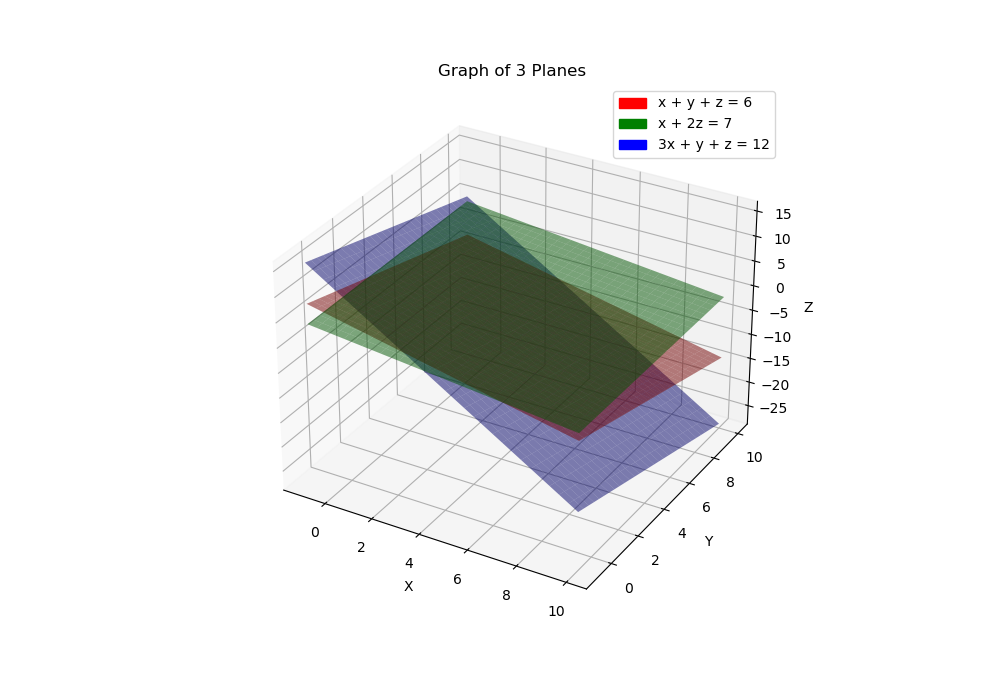
\includegraphics[width=\columnwidth, height=0.8\textheight, keepaspectratio]{Figure_11.png}     
\end{frame}
\end{document}